% -*- root: ../../DAT2-A423_Project_Report.tex -*-
\section{Steganalysis}
\label{steganalysis}
Steganalysis is the disipline of detecting information hidden with steganography and if possible, recover that information.
Because of the nature of steganography, it is not always obvious if a file has hidden information or not.
There are many different techniques used in detection of hidden data.
Some of these techniques are described below.


\subsection{Detection}
\label{Detection}
Most steganography algorithms are able to hide data without any notable visual impact on images, an example being LSB where it is not easily visible on the images where changes have been made to the pixels.
It is therefore hard if not impossible to detect if something is hidden by simply looking at the image.

Detection of hidden data is therefore done with statistical tools like looking at histograms, modified DCT coefficients and signatures of different steganography algorithms.

\paragraph*{Colour Histogram}
A colour histogram is a representation of the distribution of colours in an image. 
This can be used to detect unusual distributions of colour, which may occur when modifying the least significant bit or bits of each colour channel.

\begin{figure}
	\centering
	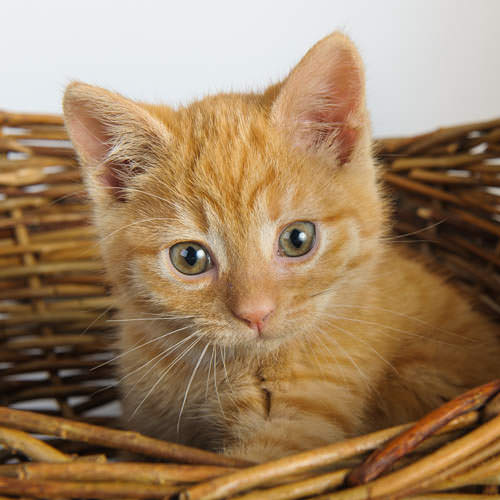
\includegraphics[width=0.4\textwidth]{figures/cover.jpg}
	\caption{Cover image. \citep{imgCover}}
	\label{fig:CoverImage}
\end{figure}

\begin{figure}
	\centering
	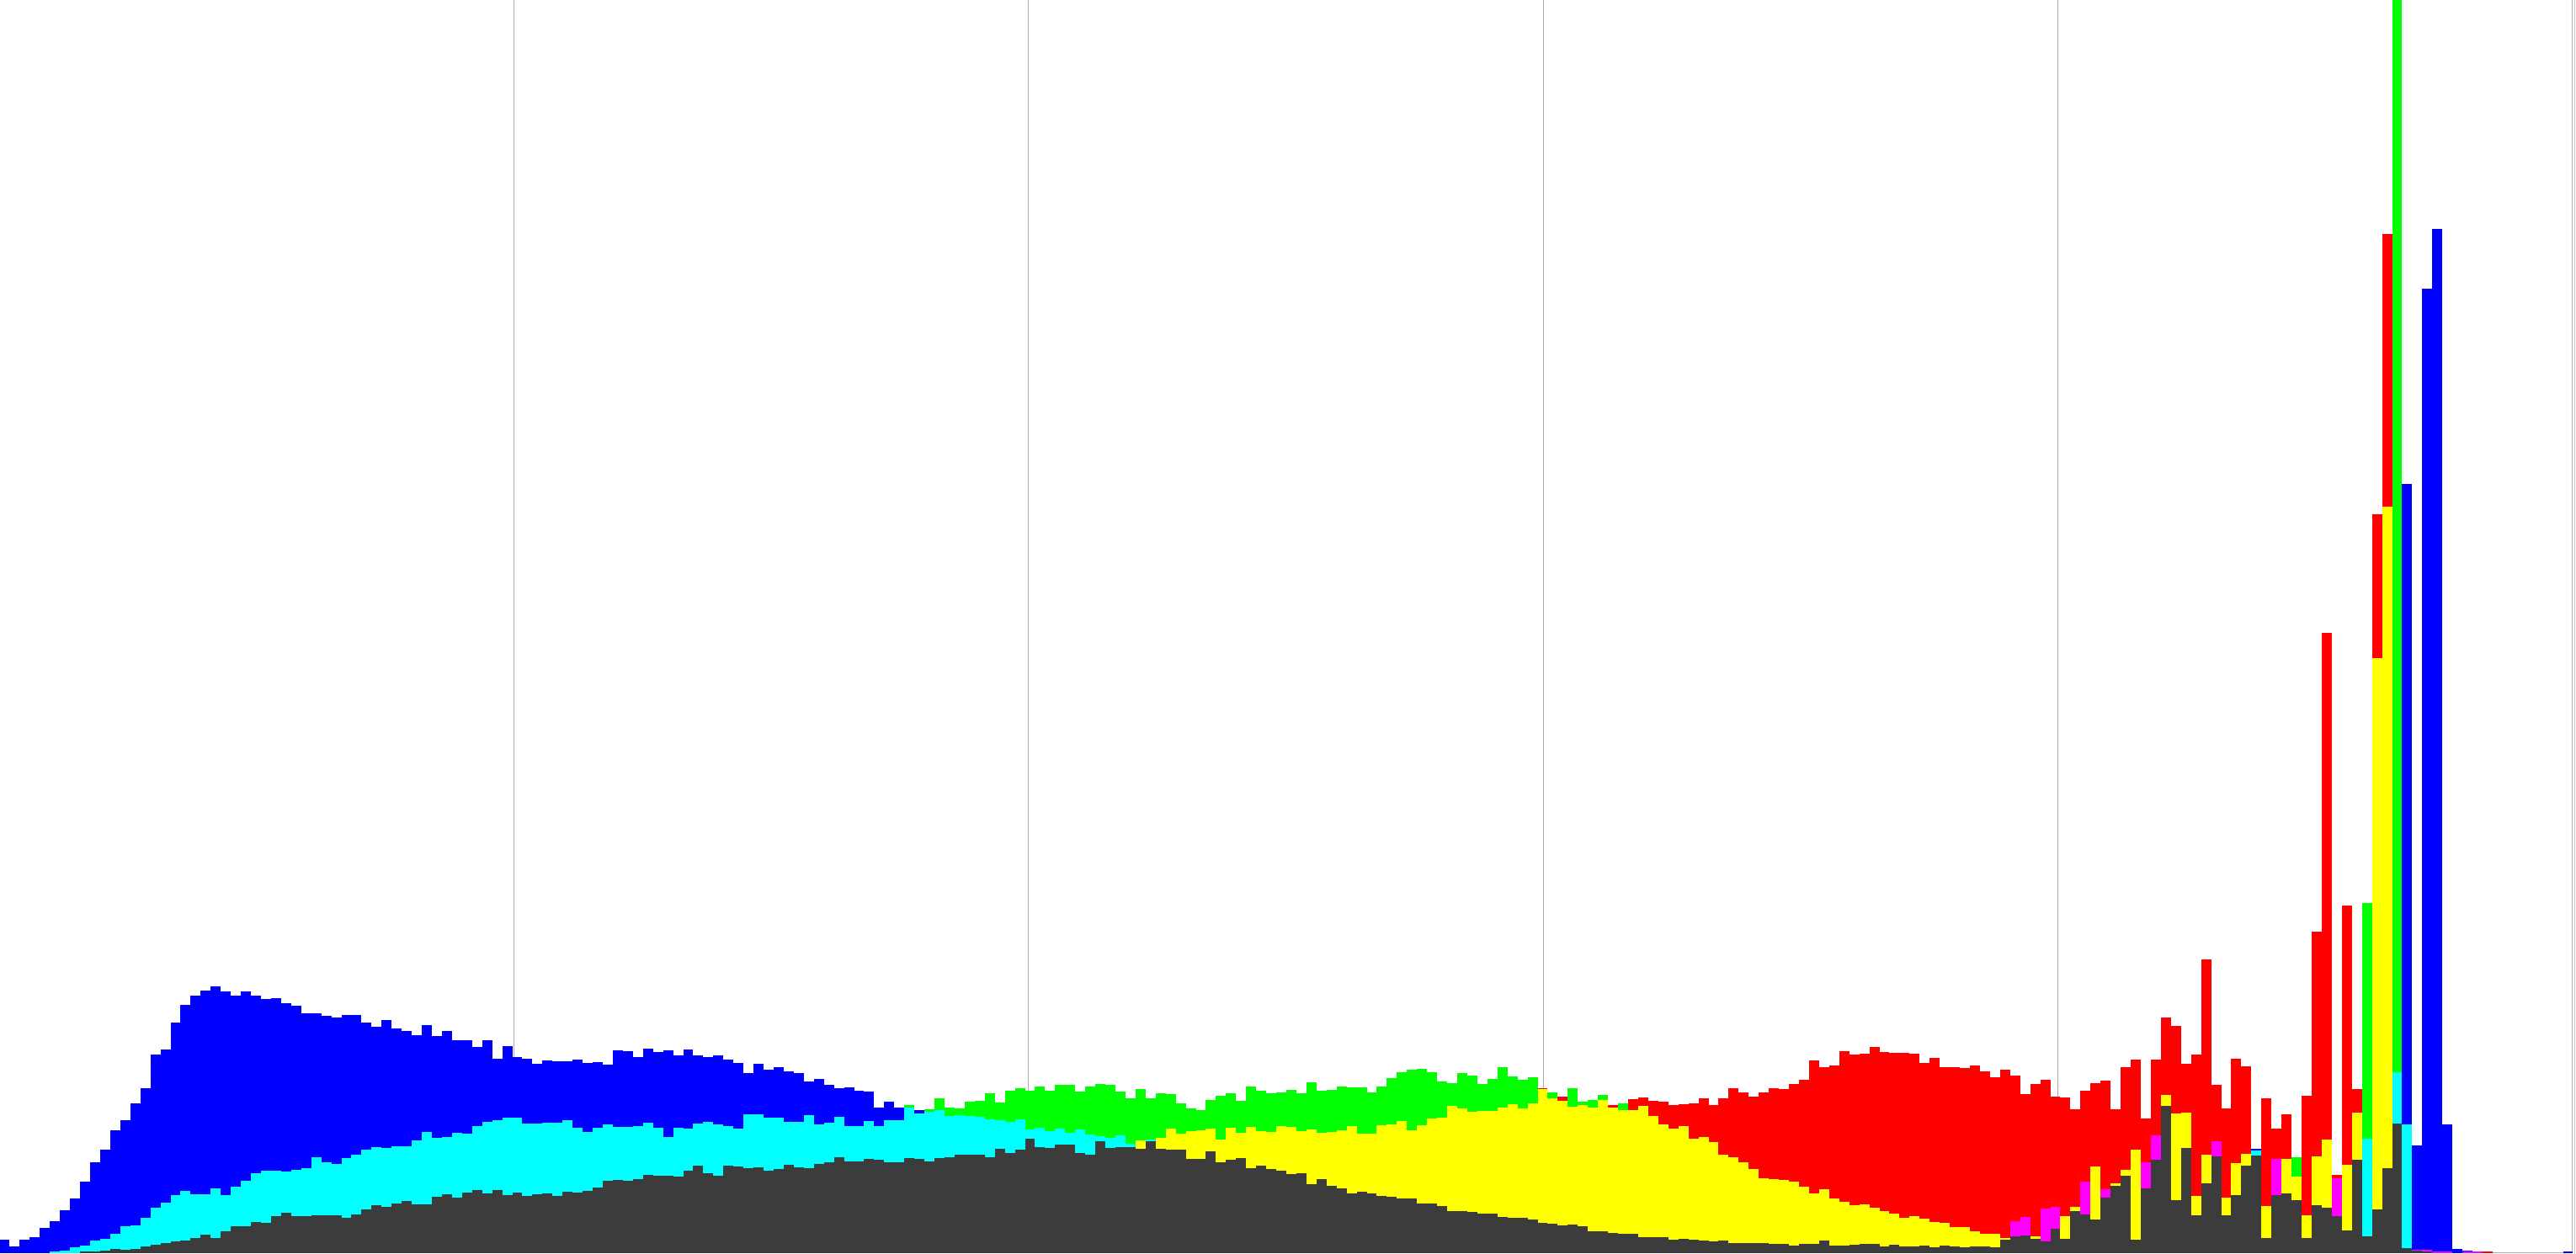
\includegraphics[width=0.6\textwidth]{figures/HistoLSBCat.png}
	\caption{Colour histogram of image shown in figure \ref{fig:CoverImage} without hidden data.}
	\label{fig:HistoWithoutLSB}
\end{figure}

\begin{figure}
	\centering
	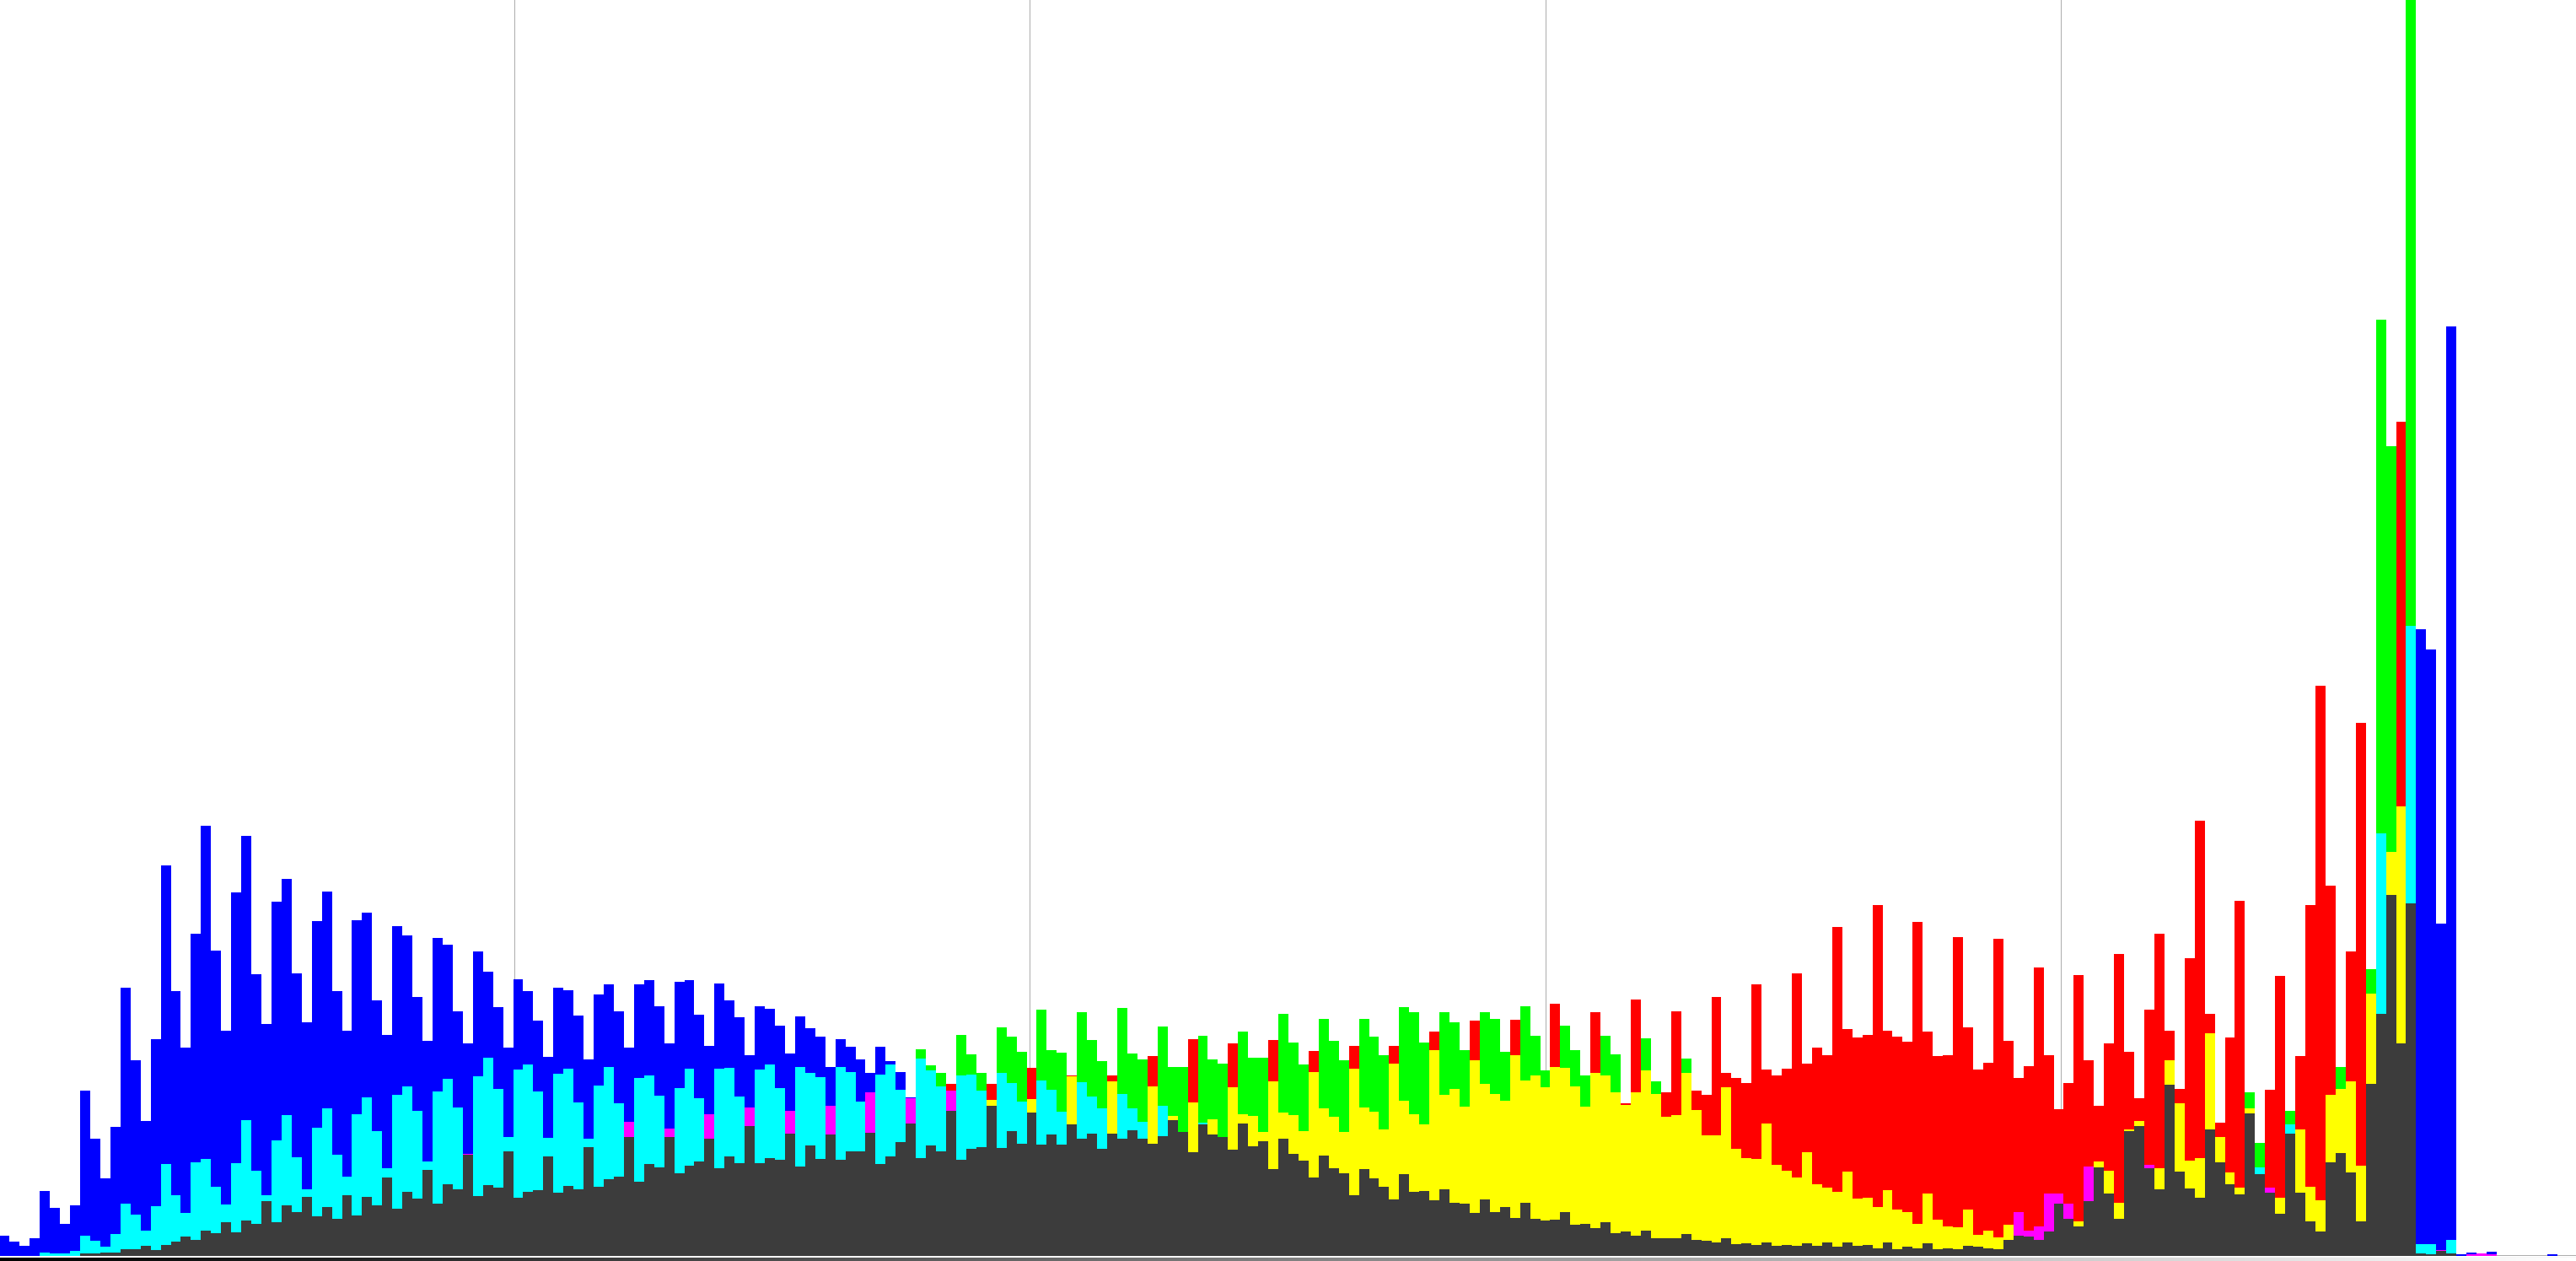
\includegraphics[width=0.6\textwidth]{figures/HistoLSBCatEncrypted.png}
	\caption{Colour histogram of image shown in figure \ref{fig:CoverImage} containing secret image hidden with LSB.}
	\label{fig:HistoWithLSB}
\end{figure}

We have our cover image shown in figure \ref{fig:CoverImage} and its respective colour histogram in figure \ref{fig:HistoWithoutLSB}.
We then hide another image in our cover image, using the implementation of LSB in section \ref{sec:lsb-implementation}. This produces a new colour histogram shown in figure \ref{fig:HistoWithLSB}.
The new stego image has quite an unusual histogram, though unfortunately we cannot be sure there is hidden data only by looking at these histograms.

This unusual histogram might just be a product of a compression algorithm.

\paragraph*{DCT coefficients histogram}
To detect if data is hidden using an algorithm which employs shrinkage, we can look at a histogram of the DCT coefficients.
When hiding data in the least significant bit of the DCT coefficients instead of just changing the bits, we can analyse each of the bits.
If the least significant bit matches our message we move on, if it does not we subtract 1 from the DCT value, if the value is negative we add 1.
This is called shrinkage.
This method results in a high amount of zeros in the DCT coefficients.
This can be seen on the comparison between figure \ref{fig:InputF5} and figure \ref{fig:outputF5}, these are histograms of DCT coefficients of figure \ref{fig:puffin}.
We can clearly see that after data has been hidden using an algorithm which uses shrinkage, as there are almost only zeros remaining.

\begin{figure}
	\centering
	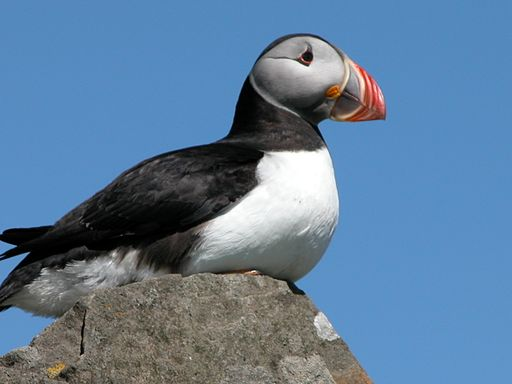
\includegraphics[width=0.35\textwidth]{figures/puffin.jpg}
	\caption{Cover image for algorithm employing shrinkage \citep{imgPuffin}}
	\label{fig:puffin}
\end{figure}

\begin{figure}
    \centering
    \begin{subfigure}[b]{0.45\textwidth}
        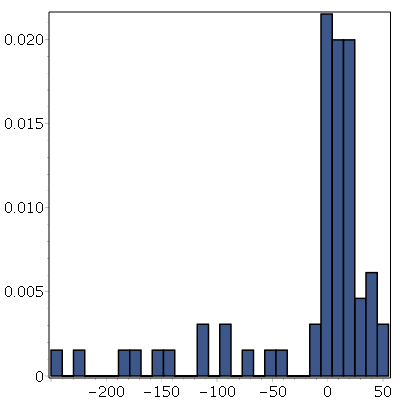
\includegraphics[width=\textwidth]{figures/inputF5.png}
		\caption{Before shrinkage}
		\label{fig:InputF5}
    \end{subfigure}
    ~ %add desired spacing between images, e. g. ~, \quad, \qquad, \hfill etc. 
      %(or a blank line to force the subfigure onto a new line)
    \begin{subfigure}[b]{0.45\textwidth}
		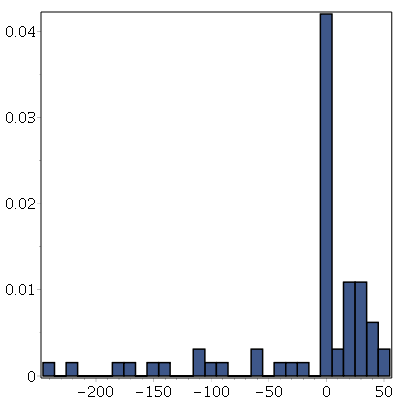
\includegraphics[width=\textwidth]{figures/outputF5.png}
		\caption{After shrinkage}
		\label{fig:outputF5}
    \end{subfigure}
    \caption{Histogram of DCT coefficients}
\end{figure}

\paragraph*{LSB enhancing}
LSB enhancing works by doing the opposite of what LSB usually does.
It eliminates all seven high-level bits for each byte. 
The least significant bit will then remain, making all bytes either 0 or 1.
These are then enhanced by setting each 0 byte to the minimum 0 and 1 to the maximum 255.
This makes the LSB of the image very visible, allowing for a visual check by simply looking for patterns.
Figure \ref{fig:hiddenAAU} shows a 24 bit BMP image with 2KB of random data hidden in it, and figure \ref{fig:LSBenhanced} is the same image LSB enhanced.
We can see that there is something hidden in the top half of the image, while the bottom half remains untouched \citep{Westfeld2000}. The reason for the logo going from blue to red is that colour of the AAU logo is (33,26,82) in RGB. The only component ending with a 1-bit, is the red component, which then gets enhanced to 255.

\begin{figure}
    \centering
    \begin{subfigure}[b]{0.45\textwidth}
		
\includegraphics[width=\textwidth]{figures/cat.jpg}
		\caption{24 bit bmp image with a 12 KB image hidden within. \citep{imgCat}}
		\label{fig:hiddenAAU}
	\end{subfigure}
	~
	\begin{subfigure}[b]{0.45\textwidth}
		
\includegraphics[width=\textwidth]{figures/Cat_LSBEnhanced.png}
		\caption{24 bit bmp image LSB enhanced.}
		\label{fig:LSBenhanced}
	\end{subfigure}
	\caption{Image of a cat before and after LSB enhancing}
\end{figure}

\paragraph*{Steganography signatures}
Unusual patterns in an image are obvious and arise suspicion, for example unused bits in the file headers or even comment headers, these might give us some insight into which algorithm was used.

\subsection{Recovery}
Recovery of data hidden with steganography is difficult. To recover the data we must know what kind of algorithm was used to hide the data.
Even if we know the algorithm used, we might still only get back meaningless data, because in addition to hiding the data, it might also be encrypted.

So the most common way of recovering hidden data is by using the same algorithm that was used to encode the image to decode the data.
